\documentclass[11pt,a4paper]{article}

\usepackage[margin=25mm]{geometry}
\usepackage{amsmath, amssymb, amsthm}
\usepackage{physics}       % \dd, \grad, \curl, \div, bra-ket
\usepackage{bm}            % \bm{} for bold-italic vectors
\usepackage{siunitx}       % \SI{3e8}{\meter\per\second}
\usepackage{booktabs}      % \toprule \midrule \bottomrule
\usepackage{array}
\usepackage{graphicx}
\usepackage{hyperref}      % LAST package

\newcommand{\Df}{D_\text{f}}
\graphicspath{{./figs/}}

\title{Reading note: physics-based simulation of soot restructuring\\
by condensation and evaporation of water}
\author{Nobuhiro Moteki}
\date{\today}

\begin{document}
\maketitle

\begin{abstract}
This note reviews the discrete element method (DEM) model of soot restructuring by Demidov, Gor and Khalizov~\cite{demidov2024}.
It also reviews the state of their public software.
The aim is to decide how compacted aggregates can be generated by a physics-based process within aggregate\_generator\_PTSA.
The contact mechanics of the model are physically grounded and partly constrained by AFM data.
The capillary driving force is a prescribed sigmoid and is not derived from the liquid.
The fraction of intact necks is prescribed, yet it controls the outcome.
A physics-based water process therefore needs three additions: a capillary bridge force derived from the meniscus, a liquid distribution from condensation and evaporation, and a neck fracture criterion.
We reproduced the restructuring results of the paper with the public code and its input files.
Aggregates from the tunable cluster-cluster aggregation of this repository give the same restructured morphology within the statistical uncertainty.
\end{abstract}

%======================================================================
\section{Scope}
\label{sec:scope}

Fresh soot aggregates have $\Df \approx 1.8$.
Coating by condensation and its evaporation make them more compact.
We want a simulation that starts from an aggregate generated by this repository, applies a water condensation and evaporation history, and returns the compacted geometry in the same HDF5 format.
This note covers the one paper read so far~\cite{demidov2024} and the software it refers to.
We read both the preprint and the published version and found no difference in the parameters or results.
Section~\ref{sec:reading} lists the papers needed next.


%======================================================================
\section{The DEM model of Demidov et al.\ (2024)}
\label{sec:demidov}

\subsection{Model}
\label{sec:model}

Monomers are rigid spheres with translational and rotational degrees of freedom.
Newton's equations for force and torque are integrated explicitly with inertia.
Each pair in contact has four springs with dashpots.
They act on normal translation, tangential translation, rolling and torsion.
The tangential, rolling and torsion springs are accumulated during the contact and rotated with the contact normal at every step.

Equation~(4) of Ref.~\cite{demidov2024} gives the relative velocity at the contact point as $\bm{v}_{ij} = \bm{v}_j - \bm{v}_i + \bm{\omega}_j \times a\hat{\bm{n}} + \bm{\omega}_i \times a\hat{\bm{n}}$, with $\hat{\bm{n}}$ pointing from $i$ to $j$.
The same form is printed in the preprint and in the published version.
The kinematics of the two contact points give instead
\begin{equation}
  \bm{v}_{ij} = \bm{v}_j - \bm{v}_i - a\,(\bm{\omega}_i + \bm{\omega}_j) \times \hat{\bm{n}} ,
  \label{eq:contact-velocity}
\end{equation}
so the order of the cross products in the printed equation is reversed.
The code (\texttt{libgran}, \texttt{contact\_force.h}) uses the normal from $j$ to $i$ and computes $\bm{v}_i - \bm{v}_j + a\,\hat{\bm{n}} \times (\bm{\omega}_i + \bm{\omega}_j)$, which agrees with Eq.~\eqref{eq:contact-velocity}.
We therefore take the printed equation as a typographical error.

Two kinds of contact exist.
A \emph{bonded} contact represents a sintered neck.
Its four springs act with force $\bm{f} = k\bm{\xi} + \eta\dot{\bm{\xi}}$, so a bonded pair moves almost as a rigid body.
A \emph{non-bonded} contact has no tensile strength.
It follows the frictional cohesive model of Luding~\cite{luding2008}, in which Coulomb's law caps the tangential, rolling and torsional springs.
In the paper the necks do not break during a simulation.
A prescribed fraction of necks is removed at random at the start.

Van der Waals attraction between monomers is the Hamaker sphere-sphere potential.
For radii $r_1$, $r_2$ and surface gap $\delta$,
\begin{equation}
  U = -\frac{A}{6}\left[\frac{2r_1r_2}{(2r_1+2r_2+\delta)\delta}
      + \frac{2r_1r_2}{(2r_1+\delta)(2r_2+\delta)}
      + \ln\frac{(2r_1+2r_2+\delta)\delta}{(2r_1+\delta)(2r_2+\delta)}\right] ,
  \label{eq:hamaker}
\end{equation}
with Hamaker constant $A = \SI{1e-19}{\joule}$.
The force diverges as $\delta \to 0$ and is cut off at a saturation distance $\delta_0 = \SI{1}{\nano\meter}$.

The capillary force between monomers $i$ and $j$ is a prescribed sigmoid of the centre distance $d_{ij}$:
\begin{equation}
  f_\text{cap} = \frac{\psi}{2}\left[1 - \tanh\bigl(\kappa (d_{ij} - d_\text{cutoff})\bigr)\right] ,
  \label{eq:sigmoid}
\end{equation}
with $\psi = \SI{1e-9}{\newton}$, $d_\text{cutoff} = \SI{56}{\nano\meter} = 4r$ and $\kappa = \SI{1.79e8}{\per\meter}$.
The force acts between every pair closer than $d_\text{cutoff}$, including pairs that are not in contact.
The authors state that $\psi$ was chosen to match the order of magnitude of literature values.

\subsection{Setup and parameters}
\label{sec:parameters}

Table~\ref{tab:demidov-parameters} lists the main parameters of the restructuring runs.
The aggregates were generated by tunable CCA (FLAGE~\cite{skorupski2014}) with $\Df = 1.8$, $k_\text{f} = 1.4$ and $N = 150$ monomers of equal radius.

\begin{table}[htbp]
  \centering
  \caption{Parameters of the restructuring simulations in Ref.~\cite{demidov2024}.}
  \label{tab:demidov-parameters}
  \small
  \begin{tabular}{>{\raggedright\arraybackslash}p{70mm}l}
    \toprule
    Quantity & Value \\
    \midrule
    Monomer radius, density & \SI{14}{\nano\meter}, \SI{1700}{\kilo\gram\per\cubic\meter} \\
    Monomers per aggregate, $\Df$, $k_\text{f}$ & 150, 1.8, 1.4 \\
    Time step, duration & \SI{5e-15}{\second}, \SI{5e-8}{\second} \\
    Bond stiffness: normal; tangential, rolling, torsion$^{a}$ & \SI{1e6}{\newton\per\meter}; \SI{1e7}{\newton\per\meter} \\
    Non-bonded stiffness (all four springs) & \SI{1e4}{\newton\per\meter} \\
    Friction coefficients: sliding, rolling and torsion & 1.0, 0.1 \\
    Hamaker constant, saturation distance & \SI{1e-19}{\joule}, \SI{1}{\nano\meter} \\
    Capillary force $\psi$, $d_\text{cutoff}$ & \SI{1}{\nano\newton}, \SI{56}{\nano\meter} \\
    Aggregates per necking fraction & 50 (49 distinct$^{b}$) \\
    Necking fractions & 0, 15, 30, 50, 70, 80, 90, 95, 98, 100\,\% \\
    \bottomrule
  \end{tabular}

  \raggedright\footnotesize
  $^{a}$ From the input files of the Supplemental Material.
  Figure~3 of Ref.~\cite{demidov2024} assigns these values to the AFM runs and \SI{1e5}{\newton\per\meter} to the restructuring runs.
  The input files do the opposite (Sec.~\ref{sec:si}).\\
  $^{b}$ The input of aggregate~7 points to the file of aggregate~5 with the same random seed.
\end{table}

\subsection{Supplemental Material}
\label{sec:si}

The Supplemental Material consists of a 10-page PDF and an archive of input files.
The PDF describes the software design and the validation tests.
The equations of motion are integrated with a leapfrog form of velocity Verlet after Kruggel-Emden et al.~\cite{kruggel2008}:
\begin{equation}
  \bm{v}_{t+\Delta t/2} = \bm{v}_{t-\Delta t/2} + \bm{a}(\bm{x}_t, \bm{v}_{t-\Delta t/2})\,\Delta t , \qquad
  \bm{x}_{t+\Delta t} = \bm{x}_t + \bm{v}_{t+\Delta t/2}\,\Delta t .
  \label{eq:leapfrog}
\end{equation}
Orientations and angular velocities are advanced in the same way.
The validation tests use two or three particles.
They show conservation of linear and angular momentum to machine precision, conservation of energy without damping, and agreement of the van der Waals force with the Hamaker potential.
The validation runs use $\Delta t = \SI{1e-14}{\second}$ and $A = \SI{1e-20}{\joule}$, which differ from the production runs.
The PDF refers to the GitHub documentation for further details, such as the rotation of the accumulated springs.

The archive contains the input files of all AFM and restructuring runs and the 50 aggregates of 150 monomers in FLAGE format.
The restructuring inputs agree with Table~\ref{tab:demidov-parameters} except for the bond parameters.
They use a bond stiffness of \SI{1e6}{\newton\per\meter} (normal) and \SI{1e7}{\newton\per\meter} (other springs) with normal damping \SI{1.25e-6}{\kilo\gram\per\second}.
The AFM inputs use \SI{1e5}{\newton\per\meter} and \SI{1.25e-7}{\kilo\gram\per\second}.
Figure~3 of the paper labels these two sets the other way round.
The time steps support the input files: the stiffer restructuring runs use the smaller step (\SI{5e-15}{\second}) and the AFM runs use \SI{5e-14}{\second}.
Pairs closer than $d_\text{crit} = \SI{1}{\nano\meter}$ are bonded before necks are removed.
The same random seed (0) selects the removed necks in all runs.

\subsection{Results}
\label{sec:results}

\begin{itemize}
  \item An AFM indentation simulation reproduces the sawtooth force curve measured on soot of about 120 monomers.
        The authors report that the peak magnitudes are set mainly by the Hamaker constant and their number mainly by the aggregate morphology.
  \item Restructuring finishes within tens of nanoseconds.
        Condensation takes milliseconds in saturators and hours in the atmosphere.
        The authors conclude that condensation and restructuring can be simulated separately.
  \item The necking fraction controls the pathway.
        With few necks, peripheral monomers collapse locally and interlock, which stops further compaction.
        With nearly all necks intact, whole branches move and the compaction is global.
  \item The text states a final coordination number of 4.48 without necks.
        Figure~8 of the paper and our reproduction give 4.85 (Sec.~\ref{sec:repro}), so 4.48 is a typographical error.
        The two-dimensional convexity of the final aggregates is 0.80--0.81 for necking fractions of 0\,\% and 70\,\%.
        Experiments report 0.75--0.87.
\end{itemize}

The authors list as limitations that the capillary model has no hysteresis of bridge formation and rupture.
They also note that it does not apply to thick coatings.
There the shrinking surface of an evaporating droplet pushes all monomers towards its centre instead of pulling pairs together.

%======================================================================
\section{Assessment for a physics-based water process}
\label{sec:assessment}

\paragraph{Contact mechanics.}
The contact model is standard DEM physics and carries rotation, which earlier models lacked.
The Hamaker constant is a material property.
The stiffness values are large enough to make bonded pairs nearly rigid, and they set the \SI{5}{\femto\second} time step.
The AFM comparison constrains the model only qualitatively, with one curve and a sawtooth shape.

\paragraph{Capillary force.}
Equation~\eqref{eq:sigmoid} contains no surface tension, contact angle or liquid volume.
It acts with the same magnitude on every pair within $4r$, whether or not a meniscus could exist there.
A physical scale follows from the maximum force of a small pendular bridge between two equal spheres in contact,
\begin{equation}
  F_\text{max} \approx 2\pi \gamma r \cos\theta ,
  \label{eq:bridge-max}
\end{equation}
where $\gamma$ is the surface tension and $\theta$ the contact angle.
For water ($\gamma = \SI{0.072}{\newton\per\meter}$) and $r = \SI{14}{\nano\meter}$ this gives $F_\text{max} \approx \SI{6.3}{\nano\newton}\,\cos\theta$.
The value $\psi = \SI{1}{\nano\newton}$ thus corresponds to $\theta \approx \ang{80}$ or to bridges that are far from their maximum.
The order of magnitude is plausible, but the force law is not derived from the liquid.

\paragraph{Necks.}
The necking fraction is the parameter that decides the outcome, and it is prescribed.
A physics-based process must decide which necks break from the capillary stress and a neck strength.

\paragraph{Scope of the runs.}
All monomers have one radius.
Only $N = 150$ was simulated.
Our aggregates are polydisperse and reach $N \sim 10^4$.

%======================================================================
\section{Software}
\label{sec:software}

The authors' code is public.
We checked the repositories on 2026-11-26.

\begin{table}[htbp]
  \centering
  \caption{Public software of E.~V. Demidov related to Ref.~\cite{demidov2024}, all under \texttt{github.com/egor-demidov/}.}
  \label{tab:software}
  \small
  \begin{tabular}{>{\raggedright\arraybackslash}p{40mm}l>{\raggedright\arraybackslash}p{80mm}}
    \toprule
    Repository & License & Content \\
    \midrule
    \texttt{soot-dem} & MIT & C++ simulation code of the paper; last update 2026-11-23 \\
    \texttt{libgran} & MIT & C++ template library for DEM used by \texttt{soot-dem} \\
    \texttt{libtimestep} & MIT & time-integration library \\
    \texttt{soot-dem-gui} & GPL-3.0 & graphical program with downloadable executables; last update 2024-11-10 \\
    \bottomrule
  \end{tabular}
\end{table}

\texttt{soot-dem} goes beyond the paper in three ways.
\begin{itemize}
  \item Neck breaking during restructuring (\texttt{restructuring\_breaking\_necks*.cpp}).
        One routine breaks a randomly chosen neck.
        Another reads neck strengths from a file.
        Tensile, shear and torsion test programs for neck strength are included.
  \item Three coating force models (\texttt{coating\_force.h}): the sigmoid of Eq.~\eqref{eq:sigmoid}, a model based on the filling angle of the liquid, and a shrinking-sphere force for thick coatings.
        We have not yet read their equations.
  \item An experimental resolved-liquid model (\texttt{capillary/}) that couples smoothed-particle hydrodynamics to the DEM.
        The authors' own status file of 2026-11-05 states that the surface-tension calibration has not passed and that the bridge force is not validated.
\end{itemize}
The code takes a single monomer radius (\texttt{r\_part}).
Polydisperse aggregates would need changes to its input and force routines.

The MIT license allows use, modification and redistribution with the copyright notice.
Code from \texttt{soot-dem} can therefore be adapted in this MIT-licensed repository.
Code from \texttt{soot-dem-gui} could only be included under GPL-3.0.
Running its executables to produce data imposes no license obligation on the data.

%======================================================================
\section{Reproduction with \texttt{soot-dem}}
\label{sec:repro}

\subsection{Setup}

We built \texttt{soot-dem} at tag \texttt{v1} (commit \texttt{7572f45}), which corresponds to the submitted article.
We ran the restructuring inputs of the Supplemental Material unchanged, except that the number of dumps was reduced from 500 to 50 (one per \si{\nano\second}).
This gives 50 aggregates at each of 10 necking fractions, or 500 runs.
Each run used one thread and took about \SI{21}{\minute}.
The runs are chaotic, and their trajectories change with the compiler and the number of threads.
Only statistics over the 50 aggregates can therefore be compared with the paper.

We repeated the 500 runs with aggregates from the tunable cluster-cluster aggregation (TCCA) of this repository.
They have the same $\Df = 1.8$, $k_\text{f} = 1.4$ and $N = 150$ monomers of equal radius.
They were written in FLAGE format and replace the published aggregates one for one.
The TCCA set has 50 distinct aggregates, whereas the published set has 49 (Table~\ref{tab:demidov-parameters}).
The radius of gyration of the monomer centres is $13.38\,r$ for TCCA and $(13.12 \pm 0.12)\,r$ for FLAGE (mean and standard deviation).
The FLAGE aggregates thus correspond to $k_\text{f} \approx 1.46$ in the same definition.
The scripts are in \texttt{analysis/dem/} of the repository.

\subsection{Morphology metrics}

The coordination number counts neighbours whose surface gap is below \SI{1}{\percent} of the monomer diameter ($0.02\,r$).
The three-dimensional convexity is $N \cdot \tfrac{4}{3}\pi r^3 / V_\text{hull}$, where $V_\text{hull}$ is the volume of the convex hull of the monomer centres.
The two-dimensional convexity is the projected area of the aggregate divided by the area of the convex hull of the projected centres.
It is averaged over the $xy$, $xz$ and $yz$ projections.
The hull of the centres reproduces the values of the paper in both cases.
The hull of the spheres or discs gives clearly smaller values.
For example, it gives 0.63 instead of 0.82 for the two-dimensional convexity without necks.
The paper defines the three-dimensional convexity as the ratio of the aggregate volume to the volume of the convex hull constructed around the aggregate.
It does not state whether the hull encloses the spheres or only their centres.

\subsection{Results}

Table~\ref{tab:repro} and Fig.~\ref{fig:dem-compare} compare the terminal values at \SI{49}{\nano\second} with Fig.~8 of the paper.
\begin{itemize}
  \item With the published aggregates, the coordination number and the three-dimensional convexity agree with the paper at all necking fractions.
        The deviations are within the 95\,\% confidence intervals and the reading uncertainty of the figure.
  \item The initial values also agree: coordination number $2.113 \pm 0.004$ against about 2.05--2.1, and convexity $0.107 \pm 0.001$ against about 0.105.
  \item The two-dimensional convexity is $0.817 \pm 0.026$ without necks and $0.779 \pm 0.023$ with \SI{70}{\percent} necks.
        The paper reports $0.81 \pm 0.03$ and $0.80 \pm 0.03$.
  \item The time evolution has the shape of Figs.~8(a) and 8(c) of the paper.
        The coordination number saturates after about \SI{10}{\nano\second}, while the convexity still grows slowly at \SI{49}{\nano\second}.
\end{itemize}
Together with Eq.~\eqref{eq:contact-velocity} and the bond parameters of Sec.~\ref{sec:si}, these results show that \texttt{soot-dem} \texttt{v1} reproduces the published restructuring results.

\begin{table}[htbp]
  \centering
  \caption{Terminal coordination number and three-dimensional convexity (hull of centres) at \SI{49}{\nano\second}.
  Means over 50 aggregates with 95\,\% confidence intervals.
  The values of the paper are read off its Fig.~8 with an uncertainty of about $\pm 0.05$ and $\pm 0.01$.}
  \label{tab:repro}
  \small
  \begin{tabular}{rcccccc}
    \toprule
    & \multicolumn{3}{c}{Coordination number} & \multicolumn{3}{c}{Convexity (3D)} \\
    \cmidrule(lr){2-4}\cmidrule(lr){5-7}
    Necks (\%) & FLAGE & TCCA & Paper & FLAGE & TCCA & Paper \\
    \midrule
    initial & $2.113 \pm 0.004$ & $2.042 \pm 0.002$ & 2.05--2.1 & $0.107 \pm 0.001$ & $0.100 \pm 0.001$ & 0.105 \\
    0   & $4.849 \pm 0.028$ & $4.843 \pm 0.029$ & 4.85 & $0.311 \pm 0.021$ & $0.295 \pm 0.023$ & 0.300 \\
    15  & $4.618 \pm 0.026$ & $4.644 \pm 0.022$ & 4.65 & $0.291 \pm 0.015$ & $0.301 \pm 0.023$ & 0.295 \\
    30  & $4.387 \pm 0.028$ & $4.384 \pm 0.025$ & 4.40 & $0.293 \pm 0.017$ & $0.297 \pm 0.017$ & 0.290 \\
    50  & $3.899 \pm 0.028$ & $3.934 \pm 0.027$ & 3.90 & $0.269 \pm 0.015$ & $0.260 \pm 0.013$ & 0.270 \\
    70  & $3.321 \pm 0.027$ & $3.314 \pm 0.024$ & 3.35 & $0.228 \pm 0.013$ & $0.227 \pm 0.012$ & 0.235 \\
    80  & $3.003 \pm 0.024$ & $2.988 \pm 0.019$ & 3.00 & $0.207 \pm 0.012$ & $0.198 \pm 0.008$ & 0.210 \\
    90  & $2.674 \pm 0.021$ & $2.665 \pm 0.020$ & 2.65 & $0.182 \pm 0.009$ & $0.174 \pm 0.010$ & 0.180 \\
    95  & $2.498 \pm 0.022$ & $2.463 \pm 0.019$ & 2.45 & $0.162 \pm 0.009$ & $0.162 \pm 0.010$ & 0.160 \\
    98  & $2.402 \pm 0.018$ & $2.365 \pm 0.015$ & 2.35 & $0.155 \pm 0.008$ & $0.151 \pm 0.006$ & 0.150 \\
    100 & $2.324 \pm 0.019$ & $2.257 \pm 0.017$ & 2.30 & $0.146 \pm 0.007$ & $0.144 \pm 0.006$ & 0.145 \\
    \bottomrule
  \end{tabular}
\end{table}

\begin{figure}[htbp]
  \centering
  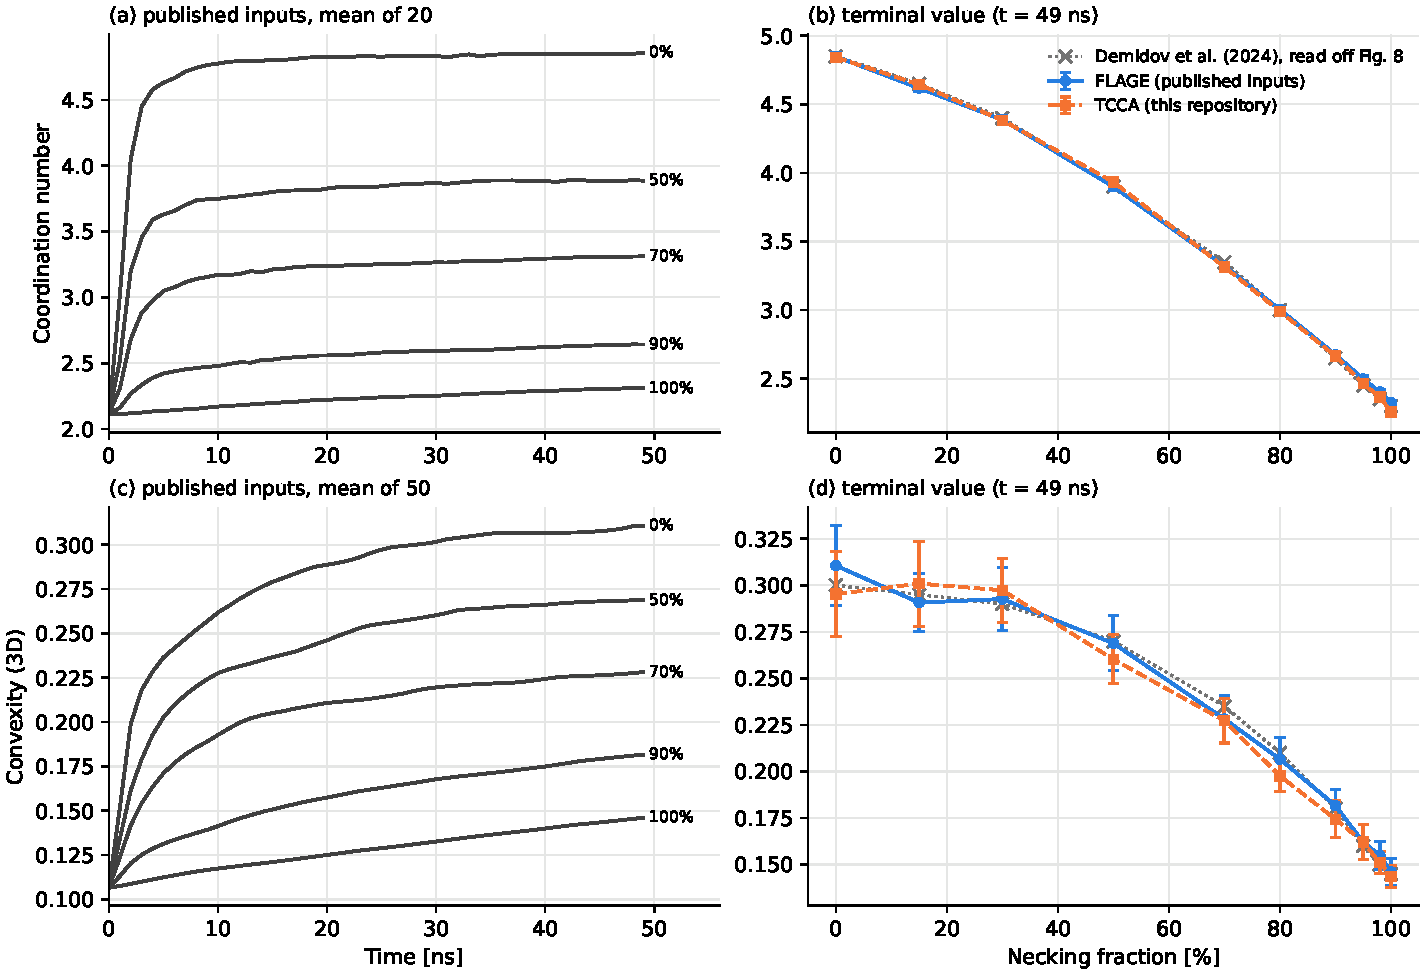
\includegraphics[width=\textwidth]{dem_compare.pdf}
  \caption{Restructuring of 150-monomer aggregates by the sigmoid capillary force.
  (a), (c) Time evolution of the coordination number and the three-dimensional convexity for the published aggregates at selected necking fractions.
  As in Fig.~8 of Ref.~\cite{demidov2024}, panel (a) averages the first 20 aggregates and panel (c) all 50.
  (b), (d) Terminal values against necking fraction for the published FLAGE aggregates and the TCCA aggregates of this repository, with 95\,\% confidence intervals.
  The dotted line shows values read off Fig.~8 of Ref.~\cite{demidov2024}.}
  \label{fig:dem-compare}
\end{figure}

\subsection{Dependence on the aggregate generator}

The TCCA aggregates restructure to the same morphology as the FLAGE aggregates.
\begin{itemize}
  \item The three-dimensional convexity shows no significant difference at any necking fraction.
        The largest difference is 1.2 standard errors.
        The two-dimensional convexity agrees as well ($0.802 \pm 0.032$ without necks and $0.780 \pm 0.023$ with \SI{70}{\percent} necks).
  \item The coordination number agrees up to \SI{90}{\percent} necks.
        At 95, 98 and \SI{100}{\percent} it is lower for TCCA by $0.036$, $0.037$ and $0.067$, or 2.4, 3.1 and 5.2 standard errors.
\end{itemize}
The difference at high necking fractions comes from the initial structure.
The TCCA aggregates start with fewer contacts (coordination number 2.042 against 2.113), because they contain fewer incidental contacts besides the tree of the aggregation.
With all necks intact the contacts are fixed, and the initial difference of $-0.071$ persists.
The increase during the run differs by only $0.004 \pm 0.023$ at \SI{100}{\percent} necks.
With fewer necks the aggregates forget their initial contacts and reach the same terminal value.
The TCCA aggregates then gain 0.03--0.10 more contacts than the FLAGE aggregates.
The \SI{2}{\percent} larger radius of gyration of the TCCA set has no detectable effect.

For $\Df = 1.8$ and $N = 150$, the choice between FLAGE and the TCCA of this repository therefore does not change the restructured morphology.
Only the number of contacts carries over when nearly all necks are intact.
The TCCA aggregates of this repository can thus serve as input for the later stages.
Whether this holds for PTSA aggregates, polydisperse monomers and larger $N$ has not been tested.

%======================================================================
\section{Implications and proposed plan}
\label{sec:plan}

The decoupling of time scales (Sec.~\ref{sec:results}) allows a quasi-static treatment.
The liquid state is advanced in steps, and the aggregate is relaxed mechanically after each step.
We propose four stages.
Each stage ends with a check before the next starts.

\begin{enumerate}
  \item \textbf{Reproduce the paper} (completed, Sec.~\ref{sec:repro}).
        Build \texttt{soot-dem} on the desktop.
        Run the published input files and reproduce the coordination number and convexity against necking fraction (Fig.~8 of Ref.~\cite{demidov2024}).
        Then replace the FLAGE aggregates by monodisperse TCCA aggregates from this repository with the same $\Df = 1.8$, $k_\text{f} = 1.4$ and $N = 150$, written in FLAGE format.
        The two runs test the code and the sensitivity to the aggregate generator.
  \item \textbf{Capillary force from the meniscus.}
        Replace Eq.~\eqref{eq:sigmoid} by the force of a pendular bridge as a function of liquid volume, gap, contact angle and surface tension.
        Add its rupture distance and hysteresis.
        First evaluate the filling-angle model already in \texttt{soot-dem}.
  \item \textbf{Liquid distribution from condensation and evaporation.}
        Compute the liquid volume at each junction from the saturation ratio, with the Kelvin effect for concave junctions~\cite{ivanova2020}.
        Evaporation reduces the volumes stepwise.
        Thick coatings need the shrinking-droplet force instead of pairwise bridges.
  \item \textbf{Neck fracture and calibration.}
        Break necks when the capillary load exceeds a neck strength.
        Calibrate the strength and contact angle against compaction measurements~\cite{chen2018,enekwizu2021,bhandari2019}.
        Then extend to polydisperse monomers and write results to HDF5.
\end{enumerate}

Whether stages 2--4 are written in C++ inside \texttt{soot-dem} or in Python and Numba in this repository is open.
Stage~1 gave the run time and showed that the aggregate generator does not matter at $N = 150$ (Sec.~\ref{sec:repro}).
The explicit integration at \SI{5}{\femto\second} over \SI{50}{\nano\second} needs $10^7$ steps, which take about \SI{21}{\minute} on one core for $N = 150$.
The force loop of \texttt{soot-dem} visits every pair of monomers (Supplemental Material), so the cost grows as $N^2$.
For $N = 10^4$ this extrapolates to about $1.5 \times 10^3$ core hours per run.
Large aggregates therefore need a neighbour list, a quasi-static energy minimisation, or both.

%======================================================================
\section{Reading list}
\label{sec:reading}

The following papers answer the open questions.
Bibliographic data are taken from the reference list of Ref.~\cite{demidov2024} unless noted.

\begin{table}[htbp]
  \centering
  \caption{Papers to read next and the question each one answers.}
  \label{tab:reading}
  \small
  \begin{tabular}{>{\raggedright\arraybackslash}p{58mm}>{\raggedright\arraybackslash}p{88mm}}
    \toprule
    Paper & Question \\
    \midrule
    Luding (2008)~\cite{luding2008} & equations of the frictional cohesive contact model \\
    Ivanova et al.\ (2020)~\cite{ivanova2020} & where water condenses in a soot aggregate (concave versus convex sites) \\
    Enekwizu et al.\ (2021)~\cite{enekwizu2021} & whether condensation, evaporation, or both restructure soot \\
    Ma et al.\ (2013)~\cite{ma2013} & restructuring during water processing (evaporation stage) \\
    Chen et al.\ (2018)~\cite{chen2018} & a single parameter that predicts compaction; calibration data \\
    Bhandari et al.\ (2019)~\cite{bhandari2019} & compaction by cloud processing in laboratory and field \\
    Schnitzler et al.\ (2017)~\cite{schnitzler2017} & dependence of restructuring on surface tension of the coating \\
    Willett et al.\ (2003)~\cite{willett2003} & hysteresis of pendular liquid bridges between spheres \\
    Rong et al.\ (2004)~\cite{rong2004} & AFM data on the mechanics of aggregates \\
    arXiv:2206.03646~\cite{arxiv2206} & mechanisms of soot restructuring and compaction (review) \\
    \bottomrule
  \end{tabular}
\end{table}

A closed-form force law for pendular bridges between spheres (for example by Willett and co-workers) is also needed for stage~2.

%======================================================================
\begin{thebibliography}{99}

\bibitem{demidov2024}
E.~V. Demidov, G.~Y. Gor, and A.~F. Khalizov,
Discrete element method model of soot aggregates,
\emph{Phys.\ Rev.\ E} \textbf{110}, 054902 (2024),
\href{https://doi.org/10.1103/PhysRevE.110.054902}{doi:10.1103/PhysRevE.110.054902}.
Preprint: arXiv:2407.14254v3.
Supplemental Material: \url{http://link.aps.org/supplemental/10.1103/PhysRevE.110.054902}.

\bibitem{kruggel2008}
H.~Kruggel-Emden, M.~Sturm, S.~Wirtz, and V.~Scherer,
Selection of an appropriate time integration scheme for the discrete element method (DEM),
\emph{Comput.\ Chem.\ Eng.} \textbf{32}, 2263 (2008).

\bibitem{luding2008}
S.~Luding,
Cohesive, frictional powders: contact models for tension,
\emph{Granular Matter} \textbf{10}, 235--246 (2008).

\bibitem{skorupski2014}
K.~Skorupski, J.~Mroczka, T.~Wriedt, and N.~Riefler,
A fast and accurate implementation of tunable algorithms used for generation of fractal-like aggregate models,
\emph{Physica A} \textbf{404}, 106--117 (2014).

\bibitem{ivanova2020}
E.~V. Ivanova, A.~F. Khalizov, and G.~Y. Gor,
Kinetic model for competitive condensation of vapor between concave and convex surfaces in a soot aggregate,
\emph{Aerosol Sci.\ Technol.} \textbf{55}, 302--315 (2020).

\bibitem{enekwizu2021}
O.~Y. Enekwizu, A.~Hasani, and A.~F. Khalizov,
Vapor condensation and coating evaporation are both responsible for soot aggregate restructuring,
\emph{Environ.\ Sci.\ Technol.} \textbf{55}, 8622--8630 (2021).

\bibitem{ma2013}
X.~Ma et al.,
Soot aggregate restructuring during water processing,
\emph{J.\ Aerosol Sci.} (2013).
Bibliographic data from a web search; volume and pages to be confirmed.

\bibitem{chen2018}
C.~Chen et al.,
Single parameter for predicting the morphology of atmospheric black carbon,
\emph{Environ.\ Sci.\ Technol.} \textbf{52}, 14169--14179 (2018).

\bibitem{bhandari2019}
J.~Bhandari et al.,
Extensive soot compaction by cloud processing from laboratory and field observations,
\emph{Sci.\ Rep.} \textbf{9}, 11824 (2019).

\bibitem{schnitzler2017}
E.~G. Schnitzler, J.~M. Gac, and W.~J\"ager,
Coating surface tension dependence of soot aggregate restructuring,
\emph{J.\ Aerosol Sci.} \textbf{106}, 43--55 (2017).

\bibitem{willett2003}
C.~D. Willett et al.,
Effects of wetting hysteresis on pendular liquid bridges between rigid spheres,
\emph{Powder Technol.} \textbf{130}, 63--69 (2003).

\bibitem{rong2004}
W.~Rong et al.,
Complementary TEM and AFM force spectroscopy to characterize the nanomechanical properties of nanoparticle chain aggregates,
\emph{Nano Lett.} \textbf{4}, 2287--2292 (2004).

\bibitem{arxiv2206}
Mechanisms of soot-aggregate restructuring and compaction,
arXiv:2206.03646 (2022).
Found by a web search; authors to be confirmed.

\end{thebibliography}

\section*{Acknowledgment}
This document was prepared with the assistance of Claude (Anthropic).
The author assumes full responsibility for the content.

\end{document}
